% $Id: preview.tex,v 1.19 1998/06/22 08:07:00 ohl Exp $
%%%%%%%%%%%%%%%%%%%%%%%%%%%%%%%%%%%%%%%%%%%%%%%%%%%%%%%%%%%%%%%%%%%%%%%%


\NeedsTeXFormat{LaTeX2e}
\documentclass[11pt]{article}
\usepackage{amsmath,amssymb,amsthm}
\usepackage[margin=1.0in]{geometry}
\usepackage{amscd}
\usepackage{epsfig}
\allowdisplaybreaks
\setlength{\unitlength}{1mm}
%%%%%%%%%%%%%%%%%%%%%%%%%%%%%%%%%%%%%%%%%%%%%%%%%%%%%%%%%%%%%%%%%%%%%%%%
\makeindex
\begin{document}
\title{\bf {PURE DATA FOUNDATION OF MATHEMATICS}}
\author{%
  Saul Youssef%
  \hfil \\
  Department of Physics \\
  Boston University \\
  youssef@bu.edu\\
}
\maketitle
\begin{abstract}
We propose an axiomatic foundation of mathematics based on the {\it finite sequence} as the foundational concept, rather than based 
on {\it logic} and {\it set}, as in set theory, or based on {\it type} as in dependent type theories.  Finite sequences lead to a concept of {\it pure data} which is
used to represent all mathematical objects.  As an axiomatic system, the foundation has only one axiom which
defines what constitutes a valid definition.  An internal {\it true/false/undecided} valued logic and an internal language are defined from the single axiom
making logic and syntax related axioms unnecessary.  Valid proof and valid computation are defined in terms of equality of pure data.  An algebra of pure data
leads to a rich theory of {\it spaces} and {\it morphisms} which play a similar role as does Category theory in classical Mathematics.  As examples and
exercise of the proposed logical structure, we address the consistency of Mathematics, and paradoxes due to G\"odel, Berry, Curry and Yablo.
\end{abstract}
%%%%%%%%%%%%%%%%%%%%%%%%%%%%%%%%%%%%%%%%%%%%%%%%%%%%%%%%%%%%%%%%%%%%%%%%

%%%%%%%%%%%%%%%%%%%%%%%%%%%%%%%%%%%%%%%%%%%%%%%%%%%%%%%%%%%%%%%%%%%%%%%%
\section{Foundation}

     Any system of reasoning must necessarily have foundational concepts which are intrinsically understood, even before a first definition.
In the case of type theories\cite{Type,Type2,HOTT,aldor}, for example, there is no definition of `type' and in Zermelo-Fraenkel Set Theory(ZFC\cite{ZFC}), there is no definition of `true', `false' or `set.'
In our case, we have one foundational undefined concept:
the {\it finite sequence}.  We assume that finite sequences and obvious statements about finite sequences are understood.  
Logic, logical values and the analogue of propositions, on the other hand, will appear as varieties of `data.'  Data is defined in terms of finite sequences as follows:
\begin{itemize}
\item {\it data} is a finite sequence of {\it codas}, and a {\it coda} is a pair of {\it data}.
\end{itemize}
If $A$ and $B$ are data, there is a natural {\it algebra of data} where $A\ B$ is the concatenation of data $A$ and data $B$ and $A:B$ is
the data formed by pairing $A$ and $B$ into a single coda.  For example, by the definition, the empty sequence of codas (written `$()$') is data.  Therefore,
the pairing of two empty sequences (written `$(:)$') is also data, and, therefore, the following sequence of three codas (:(:)(:)(:)) (:(:)) ((:):((:):)) is also data.
We refer to this as `pure data' since it is data `made from finite sequences of nothing.'
Both data in the ordinary sense (bits, bytes, language expressions) and mathematical concepts naturally appear as varieties
of pure data with simple definitions expressed in the algebra of data.  Notationally speaking, the colon operation binds from the right first and binds
less strongly than concatenation, so that $A:B:C$ means $(A:(B:C))$ and $A:B\ C$ means $(A:(B\ C))$.  We use the name `coda' both to refer 
to the pairing of two data as defined, and as the name of the axiomatic system that we are defining\cite{github}.

     In coda, answers to mathematical questions are determined by an equivalence relation `=' which is defined via a partial function from codas to data
called a `context.'  Given a context $\delta$, equality is defined by
\begin{equation}
	A\ B = \delta(A)\ B = A\ \delta(B)
\end{equation}
\begin{equation}
	A:B = \delta(A):B = A:\delta(B)
\end{equation}
for data $A$ and $B$ where the partial function $\delta$ has been extended to a function from data to data with identities.
Conceptually, $\delta$ is forced to have the same properties as the identity function on data.  Within a given context,
data $A$ is {\it empty} if $A=()$ and is {\it invariant} if $\delta(A)=A$.

     In coda, new definitions are added to a context as partial functions from codas to data.  We use a convention to guarantee that each such partial
function has it's own disjoint domain.  Let the {\it domain} of a coda $A:B$ be the data consisting of the first coda in the sequence $A$, or the empty
sequence if $A$ is empty.  A partial function mapping the all of the codas with a particular invariant domain to data is called a {\it definition}.  Definitions
can be added to a `valid' context if they do not clash, as guaranteed by the following definition.
\newtheorem*{remark}{THE AXIOM OF DEFINITION}
\begin{remark}  The empty context is valid.  If $\delta$ is a valid context and $d$ is a definition, and if no coda is in
the domain of both $\delta$ and $d$, then the union of $\delta$ and $d$ is a valid context.
\end{remark}
\noindent As an axiomatic system, coda is complete at this point.  This is quite a contrast from, for instance, ZFC which has ten axioms
even assuming predicate logic.  The reason for the simplification will become clear in the sections which follow.  In Section 3, we show
that coda contains an internal logic implicit in the structure as defined.  We adopt this logic for reasoning within coda, so we do not
need axioms related to propositional or predicate logic.  In Section 4, we show that coda also contains an internal language which can
also be defined just as with any other definition.  The language has the unusual property that all byte sequences are valid syntax,
so language and language syntax axioms are also not needed.  Axioms specifying valid ``rules of deduction'' are also not needed
because deduction, proof, and computation in coda are all determined by the above data equality.  Each of these is a merely a data sequence $A_0=A_1=A_2=\dots=A_n$,
deducing $A_n$ from $A_0$, computing $A_n$ starting with $A_0$ or proving that $A_0=A_n$, depending on one's point of view.
Unlike type systems with a Curry-Howard correspondence, proof and computation are the same thing in coda.

In the sections that follow,
`data' and `pure data' are interchangeable terms and `sequence' will always mean a finite sequence unless otherwise indicated.  Since coda
only has one axiom, we can refer to the Axiom of Definition as just `the axiom.'

\section{Atoms}

      If we have invariant data $D$ with length less than or equal to 1, we may, by the axiom,
add a definition $(D A:B)\mapsto(D A:B)$ to context provided
that $D$ has not already been used.  In this case, a coda $(D A:B)$ is called an {\it atom} for any $A$ and $B$.
Data with at least one atom in it's sequence is called {\it atomic} data, and data which is equal to $()$ is called {\it empty} data.
Equations (1) and (2) imply that empty data can not be equal to atomic data and the axiom implies that this fact remains
true independent of future definitions.  We shall use the words `always' and `never' to refer to properties that are independent of
future definition, so atomic data is `always' atomic, empty data is `always' empty and atomic data and empty data are `never' equal.

    As we shall see in Section 3, the classification of empty and atomic data is the basis for the internal logic of coda.
Atoms are also the mechanism for defining permanent data such as bits, bytes and byte strings.
Starting with an empty context, a first definition is suggested by the pure data examples above where pure data
appears to be `made of $()$ and $(:)$.'
It is clear that if we were to define $(:)\mapsto()$ all pure data would collapse to $()$.  This suggests that $(:)$ should be
mapped to $(:)$.  Since $(:)$ has domain $()$ and since $()$ is invariant, we define $(:B)\mapsto(:B)$ for any coda with
domain $()$.  This makes $(:)$ invariant as well, making it available as a domain for new definitions.
Continuing in this fashion, we define an invariant {\it 0-bit} to be $((:):)$, and an invariant {\it 1-bit} to be $((:):(:))$.
Atoms with a 0-bit domain are conventionally bit sequences and atoms with 1-bit domains are conventionally byte sequences.
This makes ordinary byte sequences available as invariant names for new definitions.  For example, the definition `pass' maps
all domains $({\rm pass}\ A:B)$ to $B$.  Depending on the situation,
it is sometimes convenient to refer to `pass' as a `command,' thinking of $B$ as
`input' and $A$ as `argument'.  Alternatively, `pass' can be thought of as a binary operator taking data $A$ and $B$ and producing data $B$.
Typical examples of definitions are shown in Tables 1 and 2.
\begin{table}
\begin{tabular}{ | l | l | l | }
Domain & Description & Action \\
\hline
pass & Pass input unchanged & (pass A:B)$\mapsto$ B \\
\hline
null & Empty data for any input & (null A:B)$\mapsto$ () \\
\hline
rev & Reverse the order of data & (rev : B)$\mapsto$ (), if B is empty \\
 &  & (rev : b)$\mapsto$ b, if b is an atom \\
 & & (rev : B C)$\mapsto$ (rev:B) (rev:A) \\
 \hline
 if & Conditional B & (if A:B) $\mapsto$ B, if B is empty \\
 & & (if A:B) $\mapsto$ (), if B is atomic. \\
 \hline
 ap & Apply argument A to each input & (ap A : B)$\mapsto$ (), if B is empty \\
  & & (ap A : b)$\mapsto$ A:b, if b is an atom \\
  & & (ap A : B C)$\mapsto$ (ap A:B) (ap A:C) \\
\hline
nat & The natural numbers & (nat : $n$)$\mapsto$ $n$ (nat\ :\ $n+1$) \\
\hline
= & Equality & $(=A:B)\mapsto$ (), if $A=B$, atomic if $A\neq B$ \\
\hline
def & Make a new definition & (def A:B)$\mapsto$ add definition (A $A'$:$B'$)$\mapsto$ B. \\
\hline
\end{tabular}
\caption{\label{ }{\it Typical definitions in coda.  Each definition is a partial function from codas to data defined on
codas with a specified domain.  When multiple actions are listed, the total action is defined by the first action
where the left hand side pattern applies.}}
\end{table}
In addition to the approximately 50 simple pre-defined definitions, coda includes a definition (def A : B) which lets one
add new definitions to a context provided that A is invariant and not already used in the context, according to the Axiom of Definition.
A important and typical family of definitions are the {\it applications} such as `ap' in Table 2.  These
are simple combinatorial operations on sequences.  Since finite sequences are understood, we presume that descriptions
such as those in Table 2 are sufficient for a clear understanding of the meaning of these sorts of definitions.  Further description and built in examples are available with the software, and the source code implementation of these is also always
short and readable.\cite{github}
\begin{table}
\begin{tabular}{| l  l  l | }
Schematic Coda & $\mapsto$ & Schematic Result \\
\hline
ap A:$b_1$ $b_2$ $b_3$ & $\mapsto$ & (A:$b_1$) (A:$b_2$) (A:$b_3$) \\
app $a_1$ $a_2$ $a_3$:B &  $\mapsto$ & ($a_1$:B) ($a_2$:B) ($a_3$:B) \\
ap2 $a$ $a_1$ $a_2$ $a_3$:B & $\mapsto$ & ($a$ $a_1$:$b_1$) ($a$ $a_2$:$b_2$) ($a$ $a_3$:$b_3$) \\
aps A:$b_1$ $b_2$ $b_3$ $b_4$ & $\mapsto$ & (A $b_1$:(A $b_2$ : (A $b_3$:$b_4$))) \\
apif A:$b_1$ $b_2$\dots & $\mapsto$ & $b_1$ (\dots if (A:$b_1$) is empty) $b_2$ (\dots if (A:$b_2$) is empty) \dots \\
\hline
\end{tabular}
\caption{\label{ }{\it Built in definitions are typically combinatoric operations on data as finite sequences.  The `ap' series are variations on the
idea of applying the `argument' A to `input' B, done in various ways.}}
\end{table}

\section{Logic}

    In the framework of coda, objects with mathematical meaning are represented as pure data.  This means that mathematical
questions will generally appear in the form
\begin{itemize}
\item[] Is data $A$ equal to data $B$?
\end{itemize}
Since data equality itself is available as a definition, $A$, $B$, and the answer to the question should be
encoded in the concrete data $(=A:B)$, including any logical interpretation of $A=B$.
This suggests that `logic' in coda should be a suitable coarse classification of data in general.  Part of the
intuitive appeal and meaning of logic is the expectation that conclusions about truth and falsity should
not change if one introduces some new definition after the fact.  In the context of coda, this means that
a logic classification must be stable under future definitions.  We already have a classification of data
that meets these criteria: the disjoint categories of empty and atomic data, suggesting the definition:
\begin{itemize}
\item data is {\it true} if it is empty, {\it false} if it is atomic and {\it undecided} otherwise.
\end{itemize}
Table 3 shows examples of this classification, including familiar binary operations from classical logic.
For instance, if data $A$ and $B$ are both either true or false then $({\rm xor}\ A:B)$ is $()$ for {\it true} and $(:)$ for {\it false} according to the standard truth
 table for the standard exclusive or operation.  On the other hand, if either $A$ or $B$ are
undecided, the data $({\rm xor}\ A:B)$ has no definitions that apply.  In effect, $({\rm xor}\ A:B)$ `waits' until both $A$ and $B$ become defined
enough to have logical values.

     Although true data is always true and false data is always false, undecided data may become true or false with added definitions.
This suggests that we are defining a two valued logic where undecided data are, in a sense, variables.  This is correct, but
not quite the compete picture because some undecided data must remain undecided independent of any added definitions.
Such {\it undecidable} data occurs, for example, in the G\"{o}del phenomenon as is discussed in Sections 7 and 8.
\begin{table}
\begin{center}
\begin{tabular}{ | c | c | }
\hline
 {\it True} & (), ({\bf pass}:), {\bf null} : a b c, ({\bf and}:), ({\bf or} a:), ({\bf xor} : a)  \\
 \hline
 {\it False} & a b c, {\bf first} 3 : a b (foo:bar), ({\bf and} a:b), ({\bf or} a:b)  \\
 \hline
 {\it Undecided} & foo:bar, {\bf pass}:foo:bar, {\bf last}:a b (foo:bar)  \\
 \hline
\end{tabular}
\end{center}
\caption{\label{ }{\it Examples of true/false/undecided data in a context where defined domains are shown with bold text.}}
\end{table}

Classical logic can be thought of as establishing at least two things: 1) defining how to reason correctly and 2) assigning logical meaning to `propositions.'
Within coda, reasoning is correct if and only if it is application of a definition in context and logical meaning is defined by data being either empty, atomic or neither.
Rather than propositions being foundational undefined entities, propositions in coda are just data and their logical values are also just data.
There may be an understandable disorientation when re-defining something
as fundamental as classical logic.  We have found that this disorientation is only temporary once one realizes that the familiar binary logical operations remain,
 and the seemingly odd class of `undecided' data fits in perfectly as `logic valued variables' and as `answers to questions that have no answers.'  Confidence may
 be gained in Sections 7 and 8 where we examine G\"{o}del phenomena and test the proposed logic against well known paradoxes.

\section{Language}

Both predicate logic with ZFC and dependent type theories are formal languages.  They have alphabets with special symbols
and axiomatic syntax rules which distinguish meaningful sentences from nonsense sentences such as ${\bf xx\forall yy\exists\exists}$.
The situation with coda is simpler in the sense that the language appears just as one more definition like any other.
The basic idea is to give textual control over the operations $A\ B$ and $A:B$ in the algebra of data.
Thus, if $x$ and $y$ are language expressions, partial functions
\begin{equation} \label{eqn}
( \{x\ \ y\} \ A : B ) \mapsto (\{x\}\ A : B)\ (\{y\}\ A : B)
\end{equation}
\begin{equation} \label{eqn}
( \{x : y\} \ A : B ) \mapsto (\{x\}\ A : B):(\{y\}\ A : B)
\end{equation}
allow specification of the two operations.  Language literals `A' and `B'
\begin{equation}\label{eqn}
(\{A\} A:B)\mapsto A
\end{equation}
\begin{equation}\label{eqn}
(\{B\} A:B)\mapsto B
\end{equation}
allow language specification of the left and right components of a coda.  There is more to the language, but not much more.  Additional partial functions
define grouping operations with parenthesis, allowing string literals with angle brackets, removing extraneous spaces and adding a bit of syntactic
sugar so that $A=B$ is interpreted as $(=A:B)$, $A*B:X$ is interpreted as $A:B:X$ and $X?$ is interpreted as $(?,X)$, making $X?$ behave like
a `variable.'  All of these partial functions are fused into a single partial function acting on all codas starting with text in curly braces.  The order of
the fusing determines the precedence of the operations.  Figure 1 shows an example of the language in use in a coda notebook\cite{github}.
\begin{figure}[h]
\centering
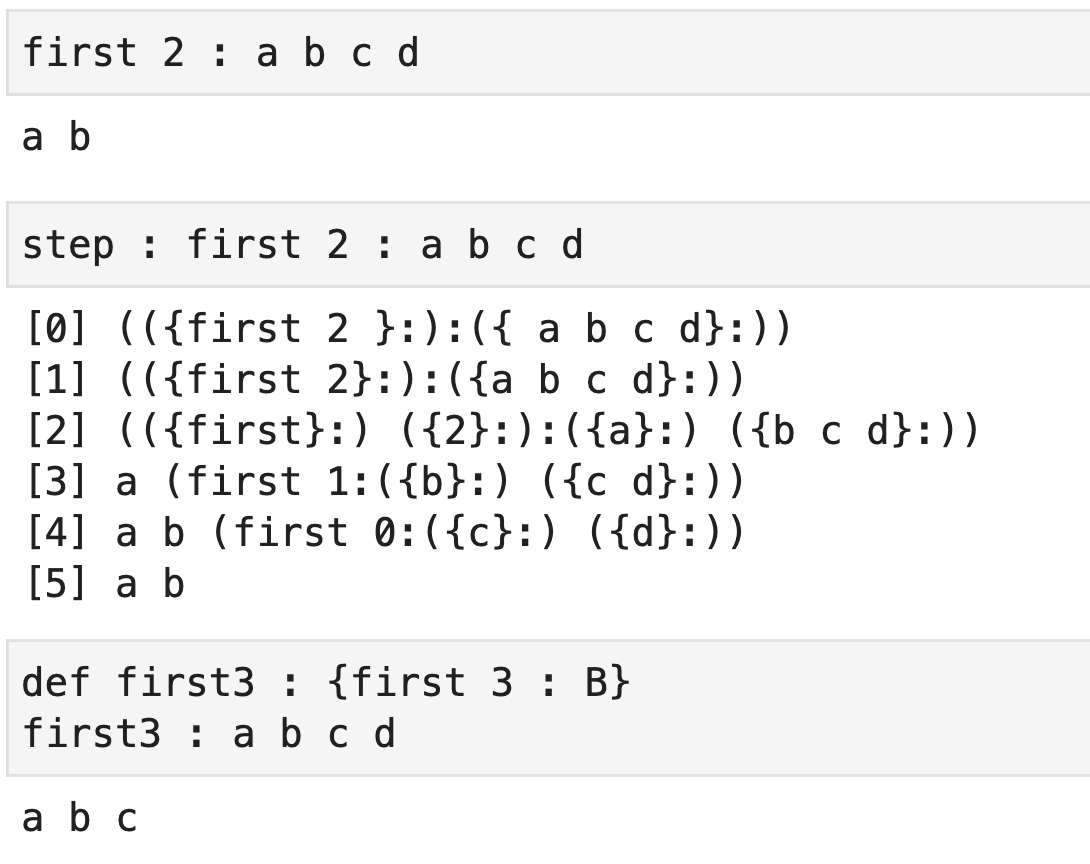
\includegraphics[width=0.5\textwidth]{fig1.png}
\caption{{\it Excerpt from a coda notebook session.  The top cell shows the `first' command selecting the first two items from the `input'
sequence of four codas.  The middle cell shows the same operation using `step' to  show the individual steps evaluating the
data `\{first 2 : a b c d\}:' which is the coda definition of the language expression `first 2 : a b c d'.  Since the language is a definition
in context like any other, language operations mix with other definitions as evaluation proceeds.  The third cell shows a typical definition added within the language.}}
\end{figure}

     The language is an intentionally minimalist wrapping of the algebra of data.
Only the characters `{\bf():\{\}=*/\ }' have language significance.  There are no reserved keywords or
special syntax for variables, functions, classes or exceptions.  The language is unusual in that any byte sequence is a valid language expression.
This means that we do not have to specify an alphabet or even define valid and invalid syntax.  There is no such thing
as invalid syntax.  The source code for the compiler and parser is small enough to be easily read and understood by
humans \cite{github}.

\section{Proof and Computation}

     As noted in Section 2, coda is both a formal system and a computational system.  As a formal system, the `sentences' of the formal system
are the pure data and the valid `rules of deduction' are that applying $\delta$ according to equations (1) and (2) preserves equality.
Given some starting data $A_0$, for instance, any chosen coda $c$ within $A_0$ can be replaced by $\delta(c)$.  This can be repeated
as desired resulting in some sequence $A_0,A_1,\dots,A_n$.  The sequence depends on the choices, but with (1) and (2) guaranteeing
$A_0=A_1=\dots=A_n$.  In this framework, the difference between a proof and a computation is merely in the strategy of where and
when to apply $\delta$.  The process of applying $\delta$ to some coda is called {\it evaluation}.  Most of the results in this paper
are computed with the very simple strategy of applying $\delta$ everywhere possible and then repeating unless and $A_i$ in the sequence
repeats.  Figures 1 and 2 show an examples of this strategy in action.  In Figure 1, the sequence converges to an atomic answer.  This does
not always happen, of course, as shown in the evaluation of the natural numbers in Figure 2.  Note what happens in Figure 2 when we compute
`the last natural number'
(last : nat : 0).  A similar result would come from computing the first of the reverse of the natural numbers (first : rev : nat : 0) or the sum of all
the natural numbers (sum n : nat : 0).  All these cases result in undecided data which is also undecidable.  Undecidable data is serving the
essential role of being the `answer to questions that have no answer.'

\begin{figure}[h]
\centering
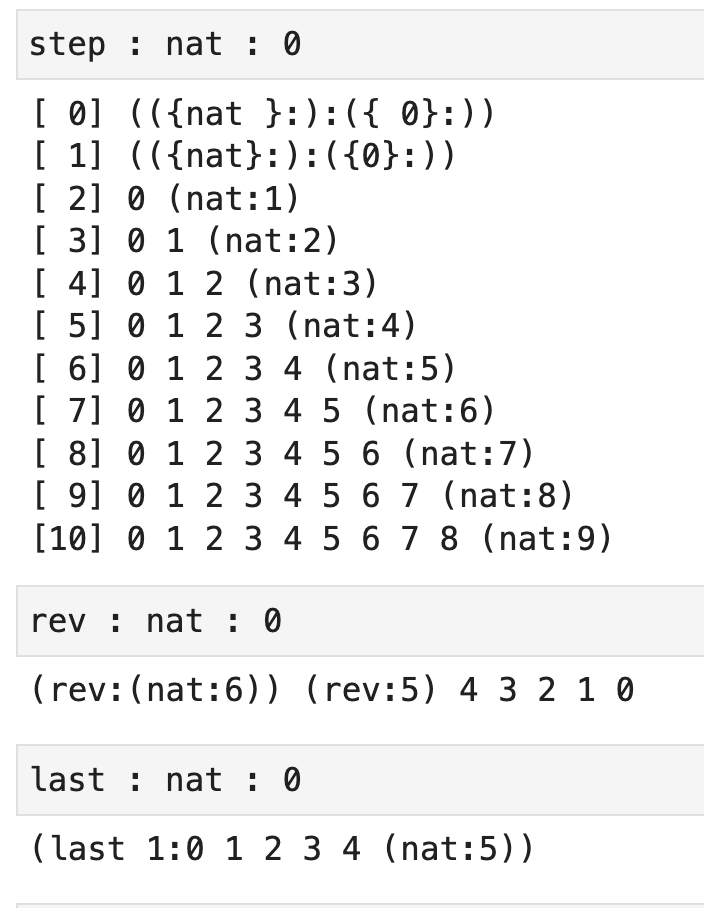
\includegraphics[width=0.4\textwidth]{nat.png}
\caption{{\it A excerpt from a coda notebook session\cite{github}.  Each cell is evaluated with the simple strategy explained in the text for up to ten
steps.  The top cell uses `step :' so each step in the strategy is displayed, showing how (nat:0) is lazily representing the natural numbers.  Note the language
elements mixing with other data in the early steps. The lower two cells show that if one computes something that has no answer, like the last natural number (last:nat:0), coda reacts by providing undecidable data as an answer.}}
\end{figure}

    The results obtained here mostly come from the above simple evaluation strategy.
We expect that there is much to be gained from a much more sophisticated approach 
where one optimizes and where and when $\delta$ is applied and where the equally valid $\delta(A)\mapsto A$ moves are included as well
as $A\mapsto\delta(A)$.  This is mostly unexplored territory as of this writing.  Coda has a couple of unusual and attractive computational properties.
Since $\delta$ is a partial function, it cannot `loop', by definition.  This means that an evaluation sequence $A_0,A_1,\dots$ may continue forever,
but each step in the sequence is guaranteed to terminate.  Also, pure data becomes like an executable in the sequence so computations or
proofs can always be saved at any point and resumed later.

\section{Spaces}

     Since the algebra of data is common to all pure data, we might expect this to be a useful common structure shared
 across multiple mathematical situations.  In this sense, the algebra of data is analogous to category theory.
 Here we take a few steps towards developing the algebra, aiming at the most natural
 way of specifying collections of data of interest called `spaces' and their associated `morphisms.'  First, a few
 preliminary definitions.
 \begin{itemize}
 \item data $A$ is {\it idempotent} if $A:A:X=A:X$ for all $X$.
 \item data $A$ is {\it distributive} if $A:X\ Y=(A:X)\ (A:Y)$ for all $X$, $Y$.
 \item data $A$ is {\it abelian} if $A:X\ Y=A:Y\ X$ for all $X$, $Y$.
 \end{itemize}
 With the algebra of data in mind, any fixed data $A$ defines a collection
\begin{equation}\label{eqn}
A:X
\end{equation}
where $X$ can be any data.  We say that $(A:X)$ {\it belongs to} $A$.  Naturally,
if $(A:X)$ and $(A:Y)$ belong to $A$, we want $(A:X)\ (A:Y)$ to also belong to $A$.  This is guaranteed if
we require
\begin{equation}\label{eqn}
A : (A : X)\ ( A: Y) = A : X\ Y
\end{equation}
for all data $X$ and $Y$.  Thus, we have the definition of a {\it space}.  Given two spaces $A$ and $B$, if
distributive data $F$ satisfies
\begin{equation}\label{eqn}
F : A : X = B : F : X,
\end{equation}
then $F$ is a mapping from $A$ to $B$ where the distributivity of $F$ guarantees that $F$ respects sequences.
In this situation, we say that $F$ is a {\it morphism} from space $A$ to space $B$.  In the case where $F$
is a morphism from space $A$ to $A$, we just say that $F$ is a `morphism of $A$.'  With abuse of pure data
equality, we say that $F$ is a morphism from $A$ to $B$ if $F*A=B*F$ where $A*B:X$ is defined to be $A:B:X$.
Each space has a special element $(A:)$ which we call the {\it neutral data} or the {\it neutral element} of a space.
If $A$ is a space and if space $B$ neutralizes each $A:X$ in the sense that
\begin{equation}\label{eqn}
A : (A:X)\ (B:X) = A : (B:X)\ (A:X) =  (A:)
\end{equation}
then we call $B$ an {\it anti-space} of $A$.  A distributive space is called a {\it type}.  
Data $F$ where $F:X$ is a space is called a {\it functor}.

Table 4 shows examples of a spaces and their corresponding morphisms.
\begin{table}
\begin{tabular}{| l | l | l | l | l |  }
Space & Action & Data &  $F*Space=Space*F$ \\
\hline
pass & A$\mapsto$A & All data & F distributive \\
null & A$\mapsto$ () & () only & F such that F:X=() \\
first & a A$\mapsto$ a & Single atoms &  F(a) for atom a \\
bool & A$\mapsto$() $or$ (:) & () or (:) &  F preserving logic \\
type n & A$\mapsto$ (n:3) (n:5) & Natural numbers &  (type n)$*$F$*$(type n) for any F \\
sum n & (n:5) (n:3)$\mapsto$ (n:8) & Natural numbers &  $F(n_1+n_2)=F(n_1)+F(n_2)$ \\
prod n & (n:5) (n:3)$\mapsto$ (n:15) & Natural numbers &  $F(n_1*n_2)=F(n_1)*F(n_2)$ \\
sort n & (n:5) (n:3)$\mapsto$ (n:3) (n:5) & Natural numbers & $n_1\le n_2 \implies F(n_1)\le F(n_2)$ \\
set n & (n:5) (n:3)$\mapsto$ equiv. classes & equiv. classes & F preserving classes \\
Sum n & $F_1\ F_2\dots F_n\mapsto F_1*\dots *F_n$ & Linear maps $n\mapsto n$ & Functorial \\
Sum & $F_1\ F_2\dots F_n\mapsto F_1*\dots *F_n$ & Linear maps  & Functorial \\
Space & $A\mapsto S_1 S_2\dots S_n$ & Spaces & ${\rm Space}*F*{\rm Space}$ for any $F$\\
Mor & $F_1\ F_2\dots F_n\mapsto F_1*\dots *F_n$ & Morphisms & Functorial \\
\hline
\end{tabular}
\caption{{\it Examples of spaces and their morphisms.  Of the spaces listed, only pass, null, type n and Space are types.
the neutral elements are (n:0) for sum n, (n:1) for prod n, the empty equivalence class for set n and pass for Sum n, Sum and Mor.  All others have neutral element ().}}
\end{table}
In general, one can think of a space as doing two things:  a) selecting data of interest and b) defining how
a finite sequence of selected data are combined to make new data in the space.
The situation with (type n) is typical.  The space (type n) constructs natural numbers from it's `input' if possible,
discarding anything that can't be converted to natural numbers represented as codas like (n:5).  (type n) is
distributive and, therefore, idempotent so natural numbers in it's input are preserved.
Since (type n) is distributive, the morphisms
of (type n) are sequence preserving arbitrary functions from naturals to naturals.
The data (sum n) is also a space, selecting the same sequences of  natural numbers as (type n), but combining
sequences with addition so that sum n : (n:3) (n:5) is equal to (n:8).  Note that a space determines it's morphisms.
A morphism of (sum n) must satisfy $({\rm sum\ n}):F:X = F:({\rm sum\ n}):X$ meaning that $F$ must be linear.
Morphisms of (sort n), on the other hand, must satisfy $({\rm sort\ n}):F:X=F:({\rm sort\ n}):X$ meaning that
morphisms of (sort n) must be order preserving functions.

     It seems promising to create an abstract theory of spaces with different additional properties.  For
 example,
\begin{itemize}
\item A space with an anti-space is a {\it pure group}.
\end{itemize}
The name is justified because the set $\{G:X | $X$\ is\ pure\ data\}$
is a group in the ordinary sense where composition, defined to be $(G:X)\times(G:Y)\rightarrow G:(G:X)\ (G:Y)$, is associative, so that
$(G:)$ the identity, and where $(G^{-1}:X)$ is the inverse of $(G:X)$ assuming $G^{-1}$ is the promised anti-space of $G$.

     An interesting possibility with spaces might be called `mathematical machine learning.'  A simple
example is illustrated in Figure 3 where we imagine that we have become interested in two different
collections of mathematical objects each just consisting of finite sequences of the atom (:).
\begin{figure}[h]
\centering
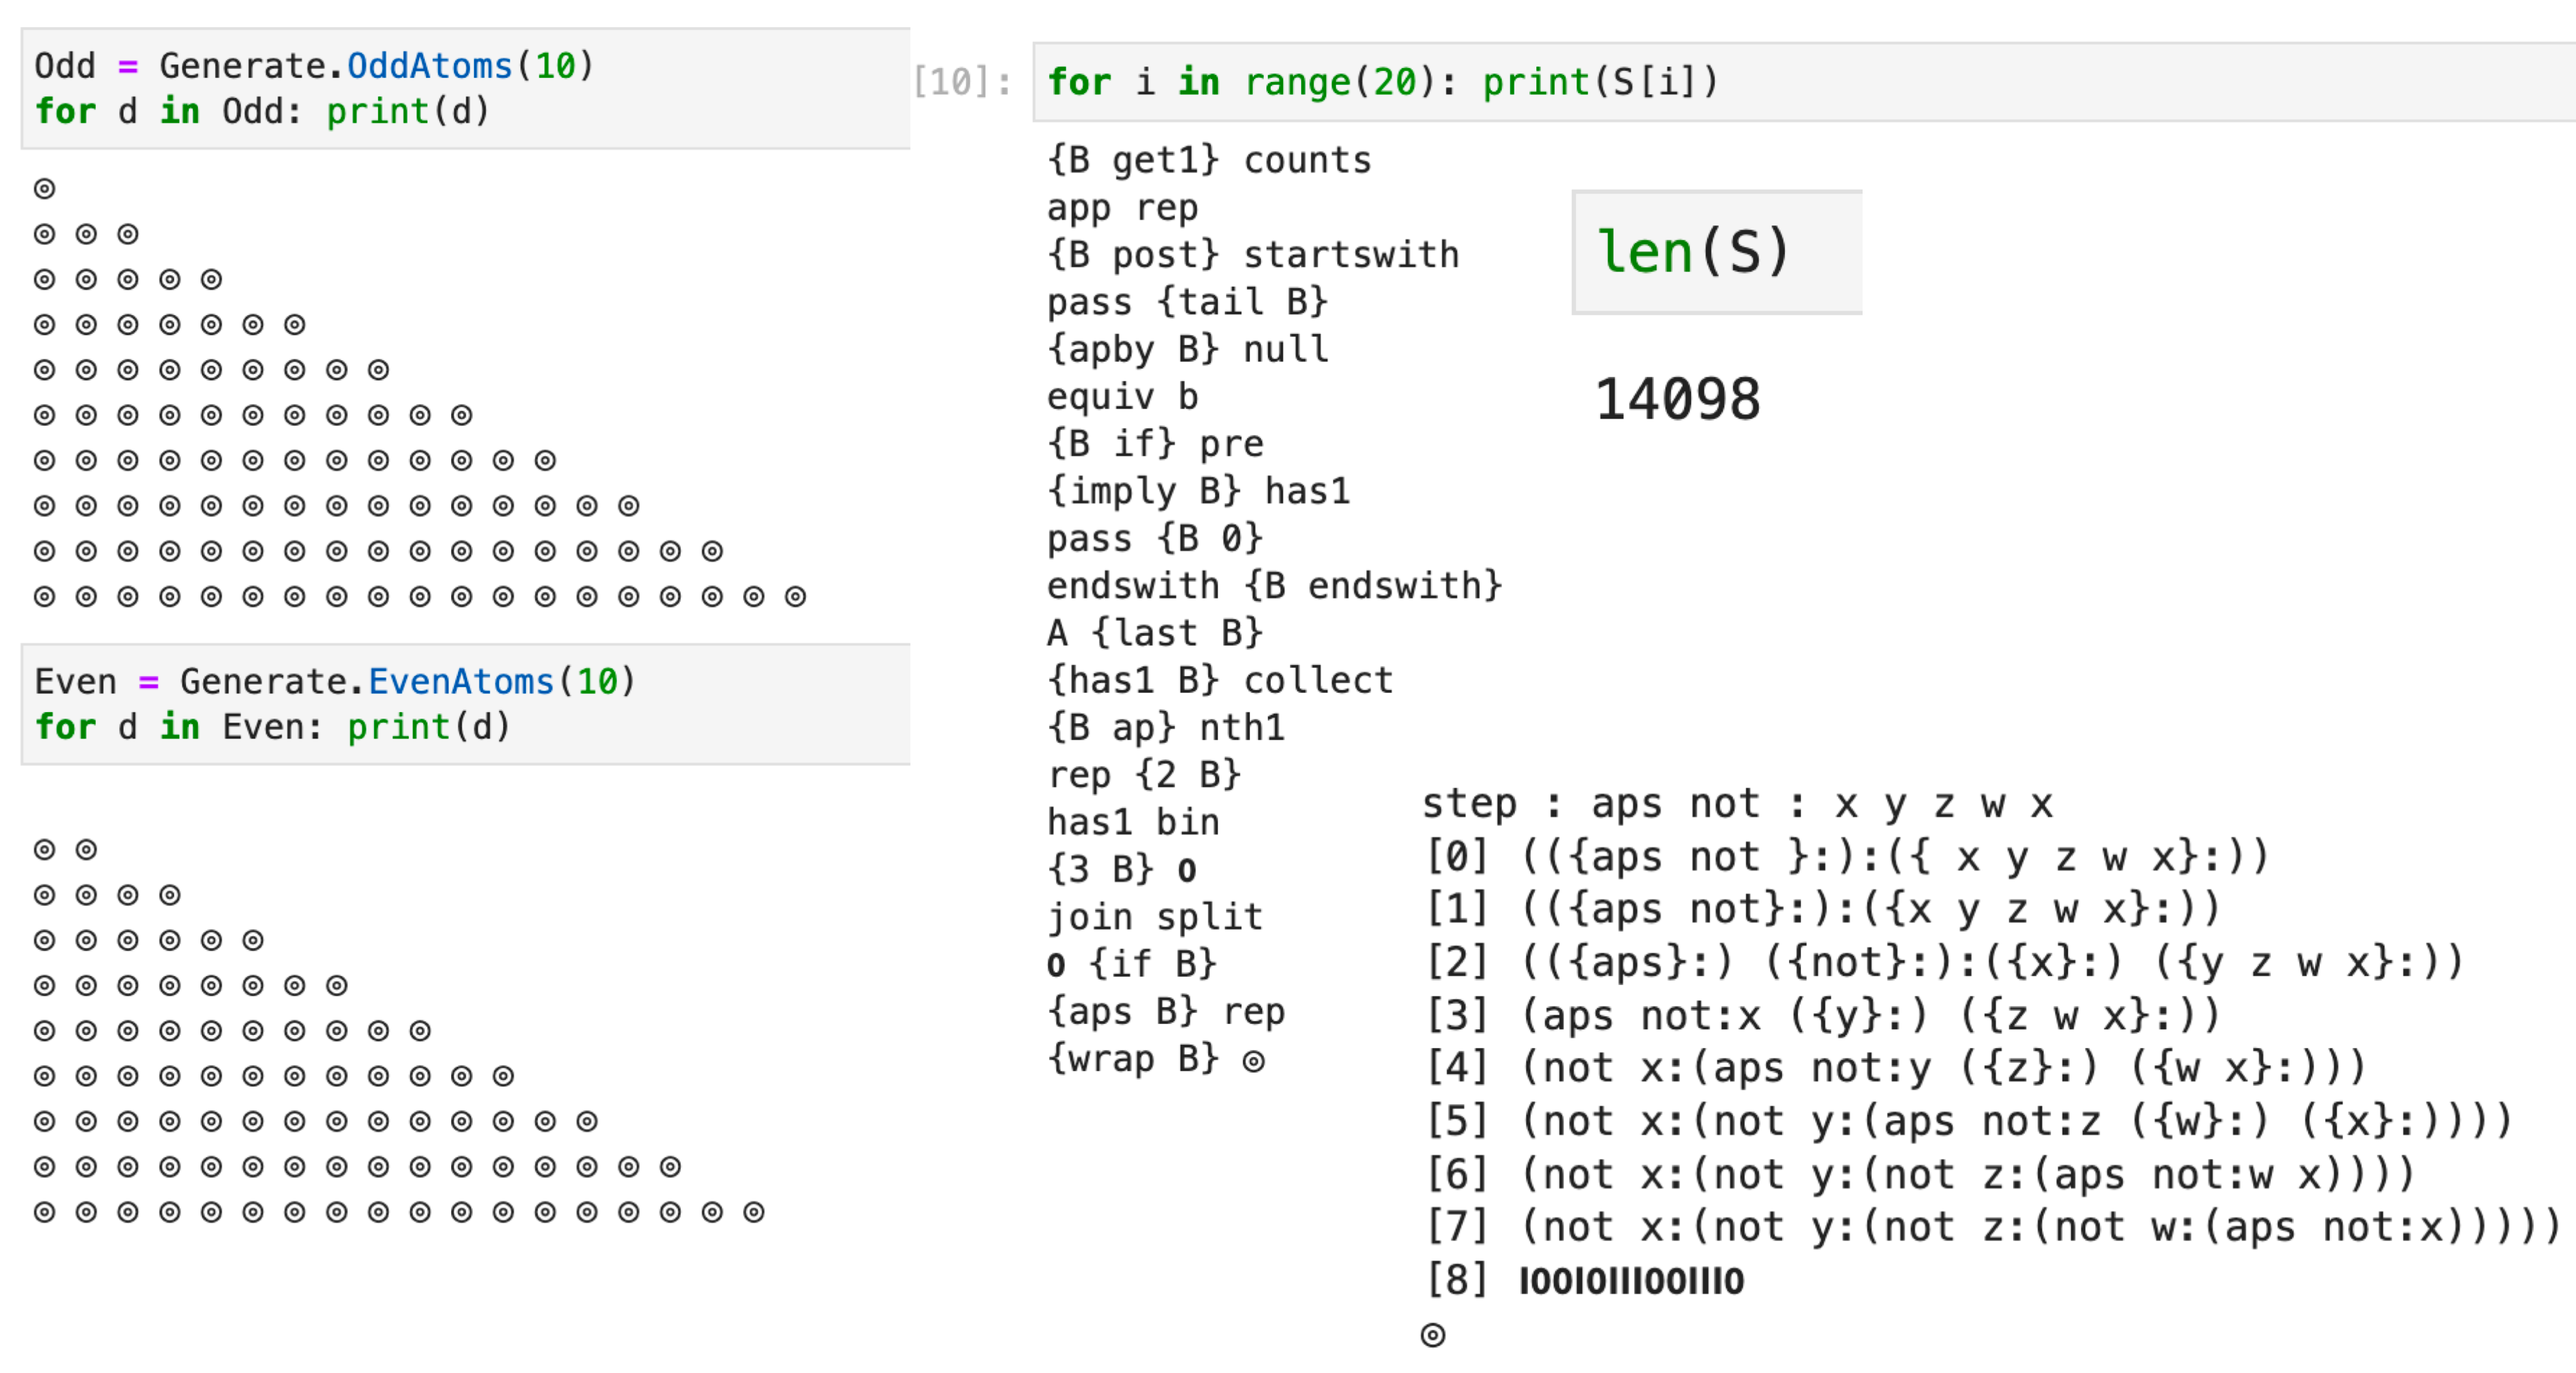
\includegraphics[width=1.0\textwidth]{machine_learning.png}
\caption{{\it Excerpt from a coda notebook session searching for a space S that distinguishes a sample of
odd numbers of (:) atoms from a sample of even numbers of (:) atoms.  Searching in a space of 18,000 data,
three candidates succeed in classifying the two samples including `aps not'.}}
\end{figure}
The difference between the two collections is that one has an odd number of atoms in each sequence and
the other has an even number.  We proceed by searching for data $A$ that succeeds in classifying
the two samples in the sense that $A:X$ have different logical values for the two collections.   A first search attempt
finds three solutions out of approximately 18,000 data, including the data  `aps not' which turns out to be true for
even numbers of (:) and false for odd numbers of (:).
Some features of the solution are interesting.
\begin{itemize}
\item The solution is clever.  It combines a combinatorial operator `aps' with a logical operator `not'
in a way that the author did not think of before doing the search.
\item The solution generalizes, since `aps not' selects data with an even number of atoms in all cases,
not just when applied to sequences of (:) atoms.
\item Although `aps not' is not quite a space, the minor modification `bool*(aps not)' is a space
in the above sense.
\item The morphisms of the space `bool*(aps not)' are interesting.  They are the functions
which preserve atomic parity of data.
\end{itemize}
Thus, just by picking out some mathematical items of interest, we have found both a way to
select similar items and have found an associated new mathematical structure.
Although this is merely a first toy example, this appears to be a strategy of general interest.

    Although the theory of spaces and morphisms clearly has something of the flavor of category theory, there are
also drastic differences.  In category theory, morphisms can be composed only if their domains and co-domains
agree.  In coda, {\it any} data $F$, $G$ and $H$ can be composed via
$X\rightarrow H:G:F:X$.  The products $F_1*F_2*\dots *F_n$ in Table 3,
for example, are always defined.  Another major structural difference
is the relationship between spaces and morphisms.  In the theory of spaces, the morphisms between space
$A$ and space $B$ are determined by $A$ and $B$.  In categories, on the other hand, there is always a choice of morphisms.  
For instance, nothing prevents one from defining a category
of real vector spaces with arbitrary functions as morphisms.  Unlike categories, coda spaces are
uniform in the sense that everything is pure data including the analogue of what would be objects, morphisms,
categories and functors in category theory.  

\section{Is Mathematics Consistent?}

     We have defined empty data to be {\it true} and atomic data to be {\it false}.  But since pure data
cannot be both true and false, we have seemingly proven that coda is consistent, seemingly
in contradiction with G\"{o}del's second incompleteness theorem.  To explore this issue,
express the consistency of coda directly in coda.  The following data
\begin{equation}\label{eqn}
{\rm ap\ \{xor\ (coda:B) : (not:coda:B) \} : allByteSequences :}
\end{equation}
logically expresses the consistency of coda in the coda language.  Here the `coda' operation maps
byte sequences to data via the onto mapping $s\mapsto (s:)$.  This means that $({\rm coda}:s)$ and
$({\rm not}:{\rm coda}:s)$ will be evaluated for each byte sequence $s$ and if they ever have the same logical
value, the overall value of (11) is false.   Although each application of `${\rm xor}\ ({\rm coda}:B) : ({\rm not}:{\rm coda}:B)$'
is true in (11), we cannot quite conclude that (11) is true because (allByteSequences:) will
eventually produce the entire byte sequence (11), which will then recursively get re-evaluated
without limit.  Thus, we have the situation where (11) is equal to
\begin{equation}\label{eqn}
() () () () () \dots ()\  (some\ undecided\ data)
\end{equation}
with endless empty sequences concatenated with forever undecided data.
We know that the undecided data will never produce an atom, but we also know that it will never disappear,
meaning that (11) never quite becomes equal to (), which is the definition of `truth.'  This appears
to be a satisfying answer.  A G\"{o}del-like limitation appears, but, it is also clear that coda
is essentially consistent in the sense that no actual contradiction can appear, even though we
cannot prove that the expression `there will be no contradiction' is true in the coda internal sense.

\section{Paradoxes}

     Here we examine logical paradoxes as a way of stress testing the proposed conception of logic.
From the coda point of view, any proposition, paradox or not, should be represented as pure data.
Any pure data can be evaluated in a given context, and coda must, therefore, give a result for 
any such proposition.

\subsection{G\"{o}del}

Recall the overall structure of G\"{o}del's second incompleteness argument\cite{Godel}.  G\"{o}del cleverly constructs a `G\"{o}del sentence' G
in Peano Arithmetic (PA) that says of itself that G is not provable in PA.  Assuming that PA is consistent in the sense
that sentences proven in PA are actually, platonically true, we proceed to reason outside of PA in platonic logic as follows.
\begin{enumerate}
\item Suppose that G is false;
\item Then G is provable in PA;
\item Since PA consistent by assumption, G is platonically true;
\item Therefore G is not provable in PA.  $\Rightarrow\!\Leftarrow$;
\item Therefore, G is true.
\end{enumerate}
Thus, we conclude that G is platonically true, but G is not provable within PA.

In coda, data $X$ is provable if and only if $X=()$, so we only have to evaluate a `G\"{o}del coda' $G?$
with definition $G?\mapsto {\rm not}:G?$.   This definition is established by
\begin{itemize}
\item let G : not : G?
\end{itemize}
in the coda language.
Evaluating $G?$ a few times, we conclude that $G?$ is equal to the undecided data
\begin{equation}\label{eqn}
{\rm (not:(not:(not:(not:(not:(not:(not:(not:(not:(({not}:):({G?}:)))))))))))}
\end{equation}
which is neither true (empty) nor false (atomic).
Since further evaluation of (13) just produces more of the same, $G?$ is an example of data which is {\it undecidable}.   At this point,
G\"{o}del's argument could be repeated to conclude that $G?$ is platonically true, but unprovable in coda.  This seems less
appealing than in G\"odel's argument, just because the self-referential source of the problem is so much more obvious.  An alternative
is to adopt coda logic platonically and just consider $G?$ to be neither true nor false.

\subsection{Berry}

     One possible attitude about, say, the liar paradox, is to avoid a mathematical paradox by just excluding
the sentence  from mathematical consideration.  After all, not all English sentences make sense mathematically, and perhaps the liar paradox is just another such sentence.  
This point of view becomes much less convincing with Berry's paradox\cite{Berry} since Berry's proposal 
 sounds like a legitimate mathematical question.
 \begin{itemize}
 \item {\it Let N = The smallest positive integer not definable in less than twelve words.}
 \end{itemize}
The problem is this.  Surely, for any positive integer $N$, $N$ either is or isn't definable in less than twelve words.
There is, therefore, a smallest such integer.  But if such an integer exists, we have succeeded in defining it in
less than twelve words.  This is a contradiction.

    To examine this issue in coda, let's agree to say that an integer is `definable in coda' if the
integer appears in the sequence $(s:)$ for some byte string $s$.  Then the following language expression
computes the maximum integer definable in coda in less than or equal to 32 characters.  Therefore,
if (14) evaluates to an integer, then any integer less than that is a Berry number.
Thus, we consider the following
\begin{equation}
{\rm max : ap\ \{coda:B\} : codes : 30}
\end{equation}
where `codes : 30' produces all character strings with length 30 or less and `max' computes the maximum integer in it's input.
The problem is that (14) is 30 characters long, so `codes : 30' will eventually produce the string `{\rm max : ap\ \{coda:B\} : codes : 30}' and 
(14) is, thus, guaranteed to remain logically undecided not matter how much it is evaluated.   
In coda, Berry's integer is undecidable. 

\subsection{Curry}

Curry's paradox\cite{Curry} is another self-referential paradox.
\begin{equation}
{\rm If\ (15)\ is\ true,\ then\ Germany\ borders\ China.}
\end{equation}
We reason as follows.  Suppose (15) is true.  Then Germany borders China.  We have thus
proved `If (15) is true, then Germany border China'.  This is exactly (15).

In coda, we can define
\begin{itemize}
\item let Curry's\_sentence : imply Curry's\_sentence? : Germany\_borders\_China?
\end{itemize}
Here (imply A:B) has the standard truth table for implication when A and B are true and false and
is undecided otherwise.  This is the same as (and A:B) or (xor A:B) or any of the 16 binary logical operators.
When evaluated in coda, `Curry's\_sentence?', as expected, is forever undecided data.  It is undecidable.

\subsection{Yablo}

     Since the Liar, Berry and Curry paradoxes have self-referential sentences, it is tempting to think
that self-referential sentences is the source of the problem.  That this is not true was shown by Yablo\cite{Yablo} who
pointed out a simple paradox with no self-referential sentences.  Consider an infinite sequence
of sentences
\begin{itemize}
\item Let $Y_1$ be $true$ if $Y_i$ is false for all $i>1$.
\item Let $Y_2$ be $true$ if $Y_i$ is false for all $i>2$.
\item Let $Y_3$ be $true$ if $Y_i$ is false for all $i>3$.
\item \dots
\end{itemize}
Suppose that $Y_n$ is true for some $n$.  Then all sentences greater than $Y_n$ are false.  But this means
that all sentences greater than $Y_{n+1}$ are also false, which means that $Y_{n+1}$ is true, contradicting
the assumption that $Y_n$ is true.  Thus, $Y_n$ cannot be true for any $n$.  But if all $Y_n$ are all false, then
$Y_0$ is true.  This is a contradiction.

     As in the previous cases, we can proceed concretely.  Introduce a definition for Yablo as follows.
\begin{itemize}
\item def Yablo : \{ap not : Yablo : skip 1 : nat : B\}
\end{itemize}
so that $({\rm Yablo}:n)$ is true if all of $({\rm Yablo}:n+1)$,\dots are not true.
\begin{figure}[h]
\centering
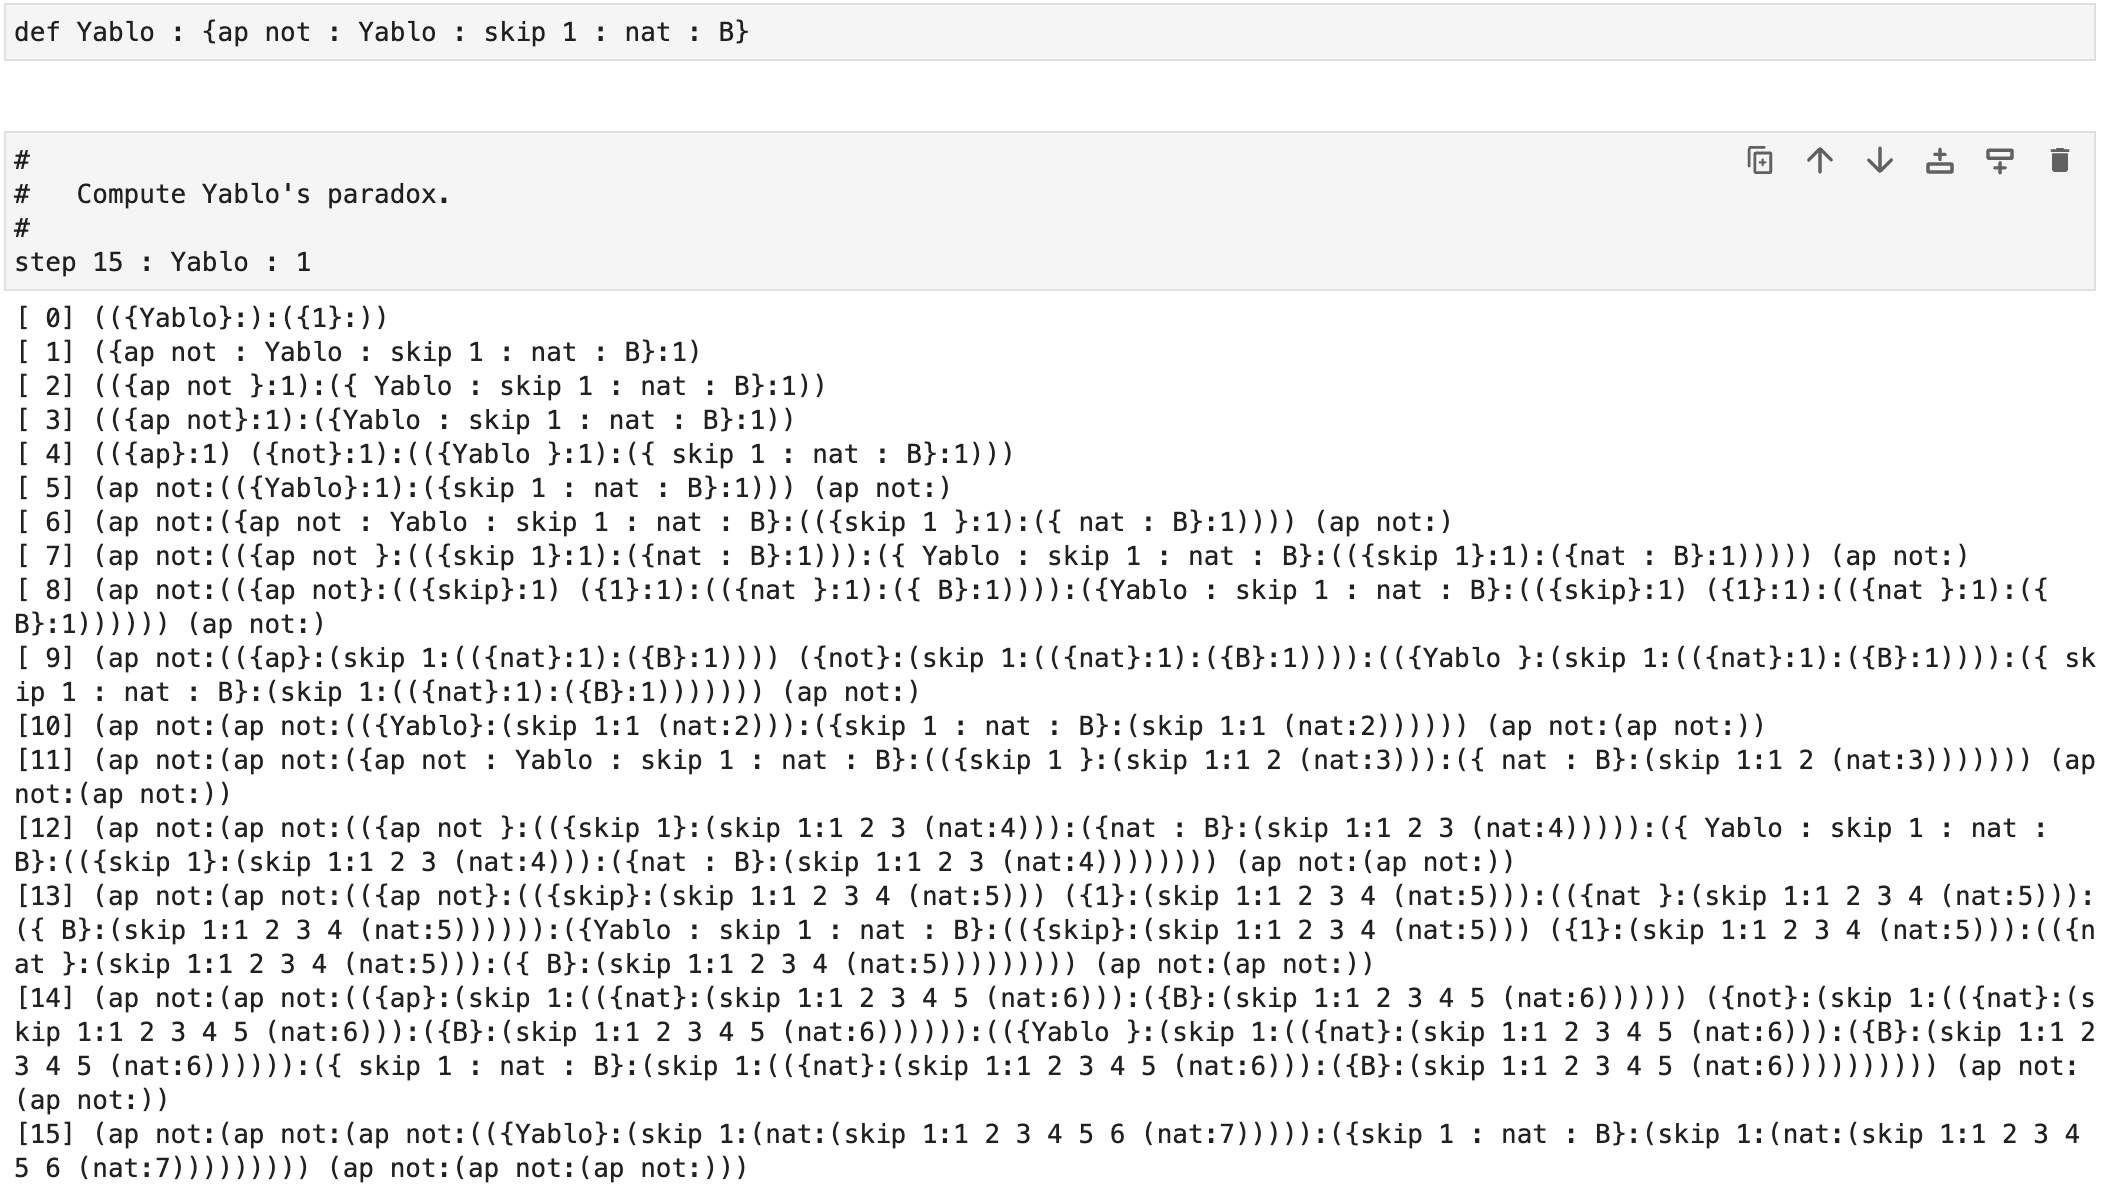
\includegraphics[width=0.9\textwidth]{Yablo.png}
\caption{{\it Evaluation of Yablo's paradox in coda.}}
\end{figure}
Figure 4 shows the evaluation of $Y_1$ in coda to depth 15.  In the G\"odel case, it is `obvious' from
the output that evaluating to greater depth will change nothing.  We have not attempted to actually
prove it, but $Y_1$ empirically remains undecided to a large depth and we fully expect that
$Y_1$ is, in fact undecidable.

It seems that in coda, paradoxes can confidently be examined as mathematical objects which
happen to have the logical value {\it undecidable}.  This makes the issue of deducing whether something
is a paradox into a concrete computational problem.  As a stress test of the coda concept
of logic, the answers to the paradoxes considered here do appear to be intuitively satisfying.

\section{Summary}

We have defined {\it coda} as an axiomatic foundation for Mathematics taking finite sequence as the starting point, rather than starting with logic, sets or types.  
In this framework, all mathematical quantities are `pure data.'  Coda has only one axiom, the `Axiom of Definition,' which defines 
what constitutes a valid definition.  The axiom induces a stable classification of pure data which we interpret as a logical system with 
empty/atomic/neither data interpreted as true/false/undecided logical values respectively.  A language is introduced via the axiom which 
gives programmatic control over pure data operations.  All byte sequences are valid language expressions so language axioms and 
axioms defining valid and invalid syntax are not needed.  Proof and computation are defined in terms of a data equality.  Unlike 
dependent type systems with a Curry-Howard correspondence, proof and computation are the same thing in coda.  A theory of {\it spaces} and 
{\it morphisms} was introduced and apparently plays a role analogous to Category Theory in classical 
Mathematics.  As an exercise of the proposed logic, we computationally address the issue of the consistency of Mathematics and paradoxes 
due to G\"odel, Berry, Curry and Yablo.  We reach a positive conclusion about the consistency of Mathematics and reach seemingly 
satisfying conclusions about the paradoxes where each paradox results in data in the undecidable category.  

    A great deal of further work seems warranted.  Only crude evaluation strategies have been attempted so far and this is an area 
where large gains are likely.  These gains are likely important for developing tools for Mathematical exploration and proof assistance.  
The example of Mathematical Machine learning in Section 6 is, at most, a hint at what's possible.  The apparently rich theory 
of spaces seems quite promising and only just barely started.  

%%%%%%%%%%%%%%%%%%%%%%%%%%%%%%%%%%%%%%%%%%%%%%%%%%%%%%%%%%%%%%%%%%%%%%%%
%%% \bibliography{jpsi}
\begin{thebibliography}{10}
\bibitem{Type} Dybjer, Peter and Erik Palmgren, {\it Intuitionistic Type Theory}, The Stanford Encyclopedia of Philosophy (Spring 2023 Edition), Edward N. Zalta \& Uri Nodelman (eds.)
\bibitem{Type2} Steve Awodey and Thierry Coquand, {\it Univalent Foundations and the Large-Scale Formalization of Mathematics}, Institute for Advanced Study, 2013.
\bibitem{HOTT} {\it Homotopy Type Theory: Univalent Foundations of Mathematics}, Institute for Advanced Study, 2013.
\bibitem{aldor} S.Watt, {\it Dependent Types and Categorical Programming}, TRICS, University of Western Ontario, 2012, available as {\rm https://cs.uwaterloo.ca/\~smwatt/talks/2012-trics-categorical.pdf}; pp. 265-270, in Handbook of Computer Algebra J. Grabmeier, E. Kaltofen, V. Weispfenning (editors) , Springer Verlag, Heidelberg 2003 , ISBN 3-540-65466-6; S.Youssef, {\it Prospects for Category Theory in Aldor}, 2008, {\rm https://physics.bu.edu/~youssef/aldor.pdf}.
\bibitem{ZFC} Bagaria, Joan, {\it Set Theory}, The Stanford Encyclopedia of Philosophy (Spring 2023 Edition), Edward N. Zalta \& Uri Nodelman (eds.)
\bibitem{github} An implementation of coda in Python is available at github.com/Saul-Youssef.  The software include Python access, a command line 
interface and a Jupyter notebook kernel plug-in.  
\bibitem{egg} The coda language is a descendent of {\it egg}.  See Saul Youssef, John Brunelle, John Huth, David C. Parkes and Margo Seltzer {\it Minimal Economic Distributed Computing}, arXiv:0902.4730.  J. Brunelle et al., In GECON 2006: Proceedings of the 3rd International Workshop on Grid Economics and Business Models, Singapore, 16 May 2006, ed. H. Lee, and S. Miller. Singapore; Hackensack, NJ: World Scientific.
\bibitem{Curry} Shapiro, Lionel and Jc Beall, {\it Curry’s Paradox}, The Stanford Encyclopedia of Philosophy (Winter 2021 Edition), Edward N. Zalta (ed.)
\bibitem{Godel} Raatikainen, Panu, {\it Gödel’s Incompleteness Theorems}, The Stanford Encyclopedia of Philosophy (Spring 2022 Edition), Edward N. Zalta (ed.)
\bibitem{Yablo} S. Yablo (1985). {\it Truth and reflection}. Journal of Philosophical Logic. 14 (2): 297–348. doi:10.1007/BF00249368.
\bibitem{Berry} Nicholas Griffin (2003-06-23). {\it The Cambridge Companion to Bertrand Russell}. Cambridge University Press. p. 63. ISBN 978-0-521-63634-6.
\end{thebibliography}
%%%%%%%%%%%%%%%%%%%%%%%%%%%%%%%%%%%%%%%%%%%%%%%%%%%%%%%%%%%%%%%%%%%%%%%%
\end{document}
